\section{Ejercicio 7}

\subsection{Consideraciones}

Para evaluar el rendimiento del scheduler \textbf{Round Robin}, consideramos las siguientes métricas:

\begin{itemize}
  \item Eficiencia: el porcentaje del tiempo consumido realizando trabajo útil (ejecutando tareas) sobre la totalidad del tiempo de ejecución, el cual incluye también el costo de cada cambio de contexto, migración entre núcleos y ejecución de la tarea IDLE.
  \item Rendimiento: la cantidad de procesos terminados por unidad de tiempo.
\end{itemize}

\begin{minipage}[t]{0.5\textwidth}
  \begin{tarea}[H]
    \vspace*{2mm}
    \begin{verbatim}
    @0:
    TaskBatch 50 3
    TaskBatch 50 10
    TaskBatch 50 20
    TaskBatch 100 3
    TaskBatch 100 10
    TaskBatch 100 20
    \end{verbatim}
    \vspace*{-5mm}
  \caption{Lote de tareas para evaluar el scheduler \textbf{Round Robin}.}
  \label{fig:lote-ejercicio-7}
  \end{tarea}
\end{minipage}\\\\

Para analizar la eficiencia y rendimiento del scheduler, se realizaron mediciones sobre la ejecución de un conjunto de tareas determinado (presentado en el Lote \ref{fig:lote-ejercicio-7}), utilizando una cantidad variable de núcleos y valores de \textit{quantum} respectivos.

Las mediciones para determinar eficiencia consistieron en un conteo de la cantidad total de ciclos de CPU consumidos por las tareas, ignorando aquellos utilizados por cuestiones propias del scheduling. En el caso multicore, se contempló con debida multiplicidad la cantidad total de ticks de ejecución; concretamente:

$$eficiencia = \frac{ciclos\;consumidos\;por\;tareas}{ciclos\;hasta\;terminar\;el\;lote * \#CPU's}$$

Por otro lado, dado que la cantidad de procesos está fijada por el tamaño del lote, la evaluación de rendimiento simplemente consistió en medir el tiempo total consumido para completar el lote; a menor tiempo, mejor rendimiento:

$$rendimiento = \frac{6}{ciclos\;hasta\;terminar\;el\;lote}$$

\subsection{Procedimiento}

Se realizaron experimentos utilizando 1, 2, 3 y 4 núcleos, manteniendo siempre fijo el costo de cambio de contexto y migración de procesos en 1 y 2 ticks, respectivamente. En cada caso, medimos la eficiencia y el rendimiento del scheduler al ejecutar el lote según las consideraciones de la sección previa, alternando los valores de \textit{quantum} en un rango lineal.

Para los casos multicore, en primer lugar se utilizó el mismo valor de \textit{quantum} para todos los núcleos, con la finalidad de evaluar el comportamiento general en función de valores cada vez mayores de ticks por turno. Luego, simulamos casos con \textit{quantums} diferentes tomados de forma pseudo-aleatoria, procurando estimar la eficiencia y rendimiento promedio para el lote y la configuración dada.

\subsection{Resultados y conclusiones}

En la figura \ref{fig:rendimiento-comparacion} presentamos un gráfico de rendimiento en función del valor de \textit{quantum} utilizado, configurando todos los núcleos con el mismo valor. Se observan en un mismo eje las curvas obtenidas para las distintas cantidades de núcleos, dentro de el intervalo $\textit{quantum} = 1, ..., 70$. Se escogió este intervalo dado que las curvas se mantienen constantes para valores de \textit{quantum} mayores.

\begin{figure}[h!t]
  \centering
  \makebox[\textwidth][c]{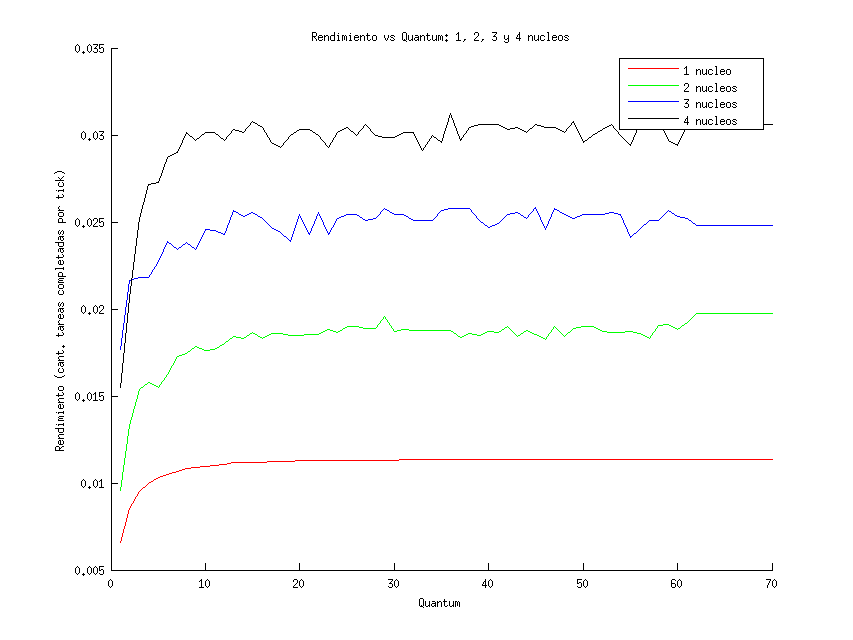
\includegraphics[width=1.1\textwidth]{graphics/ej7_rendimiento_comparacion.png}}%
  \caption{Gráfico de rendimiento en función de \textit{quantum} para el Lote \ref{fig:lote-ejercicio-7} con scheduling \textbf{Round Robin}.}
  \label{fig:rendimiento-comparacion}
\end{figure}

El gráfico muestra una tendencia de crecimiento en el rendimiento al incrementar el valor de \textit{quantum} para todas las curvas, aunque a mayor cantidad de núcleos el comportamiento es más errático. En el caso de 1 núcleo, la curva es creciente y se estabiliza en el valor de rendimiento máximo, mientras que para los demás casos existen valores que generan un mejor rendimiento que el valor de estabilización, si bien la diferencia es de pocas unidades porcentuales. Adicionalmente, se observa que a mayor cantidad de núcleos, mejor rendimiento en general; esto es esperable ya que al tener más unidades de procesamiento es razonable que el lote sea completado en menor cantidad de ticks.

Luego, en la figura \ref{fig:rendimiento-comparacion} se incluye un gráfico de eficiencia en función del valor de \textit{quantum} utilizado, nuevamente configurando todos los núcleos con el mismo valor. Las curvas obtenidas para las distintas cantidades de núcleos se superponen en un mismo eje, dentro del mismo intervalo que el caso anterior.

\begin{figure}[h!t]
  \centering
  \makebox[\textwidth][c]{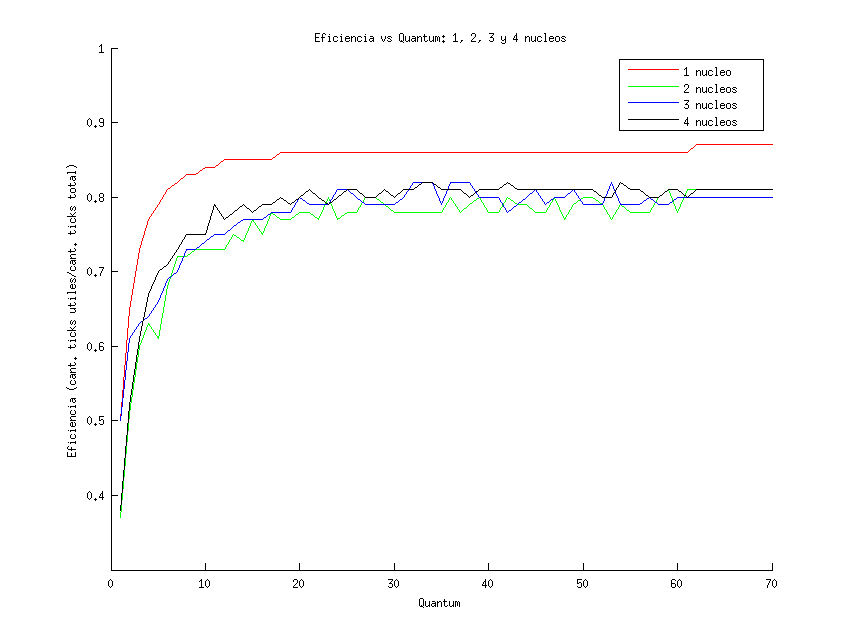
\includegraphics[width=1.1\textwidth]{graphics/ej7_eficiencia_comparacion.png}}
  \caption{Gráfico de eficiencia en función de \textit{quantum} para el Lote \ref{fig:lote-ejercicio-7} con scheduling \textbf{Round Robin}.}
  \label{fig:eficiencia-comparacion}
\end{figure}

En este caso observamos una tendencia de incremento en la eficiencia cuanto mayor sea el \textit{quantum}, si bien los casos multicore no muestran curvas estrictamente crecientes. De todas formas, el máximo de cada curva nuevamente se halla muy cercano en valor a la eficiencia estable al final del intervalo.

Las mediciones de eficiencia no muestran una correlación trivial con la cantidad de núcleos, siendo el caso de 1 núcleo el de mejor eficiencia y el de 3 núcleos el de peor. Esto posiblemente se deba a la influencia de los costos de cambio de contexto y migración de procesos, ya que al agregar núcleos se incrementa la cantidad de tareas que se pueden procesar simultáneamente, pero se también la posibilidad de tener que realizar migraciones cuando los procesos generan llamados bloqueantes de entrada/salida.

La distibución pseudo-aleatoria de \textit{quantums} para los casos multicore no arrojaron resultados destacables, mostrando en términos generales un rendimiento y eficiencia peores que las mejores configuraciones con \textit{quantums} congruentes. Por lo tanto, en términos de la eficiencia y el rendimiento de ejecución, en el caso particular del lote estudiado es beneficioso tomar valores amplios de \textit{quantum}, pudiendo utilizarse el mismo para todos los núcleos. Tomando valores mayores que el punto de estabilización (cercano a $70$) se garantiza una eficiencia y rendimiento muy cercanos al óptimo (en el caso de un único núcleo, es efectivamente el óptimo).

Por último, es importante destacar que las métricas elegidas consideran al lote en su totalidad, beneficiandose de valores grandes de \textit{quantum} ya que estos minimizan las pérdidas de tiempo conmutando tareas y realizando migraciones entre nucleos. No obstante, se ignora completamente cuestiones de fairness o repartición justa de tiempo entre las tareas, las cuales se ven negativamente afectadas al tomar dichos valores de \textit{quantum}.
